\documentclass[a4paper, 11pt]{article}
\usepackage{graphicx}
\begin{document}
\section{•}
Since there is no explicit/specific question or work assignment in this task, I'll simply state a few observations for the given system \textit{tipper} and then change certain traits of said system to alter those previous observations. This will show my understanding of fuzzy logic concepts and the usage of \textit{MATLAB's} corresponding designer. With these basics out of the way, I'll hopefully be able to keep the description of task 2's new system somewhat concise and to the point.

\subsection{Selection of input and output}
Currently, there are 2 input variables (service and food) which are used to determine the value of a single output variable (tip). This is a very logical system since service and food are probably the biggest factors for most tippers out there. To add another reasonable input variable to this setup, one could imagine a tipper who also desires a nice ambience for a generous tip. Adding \textit{ambience} results in the following system:

\begin{figure}[ht]
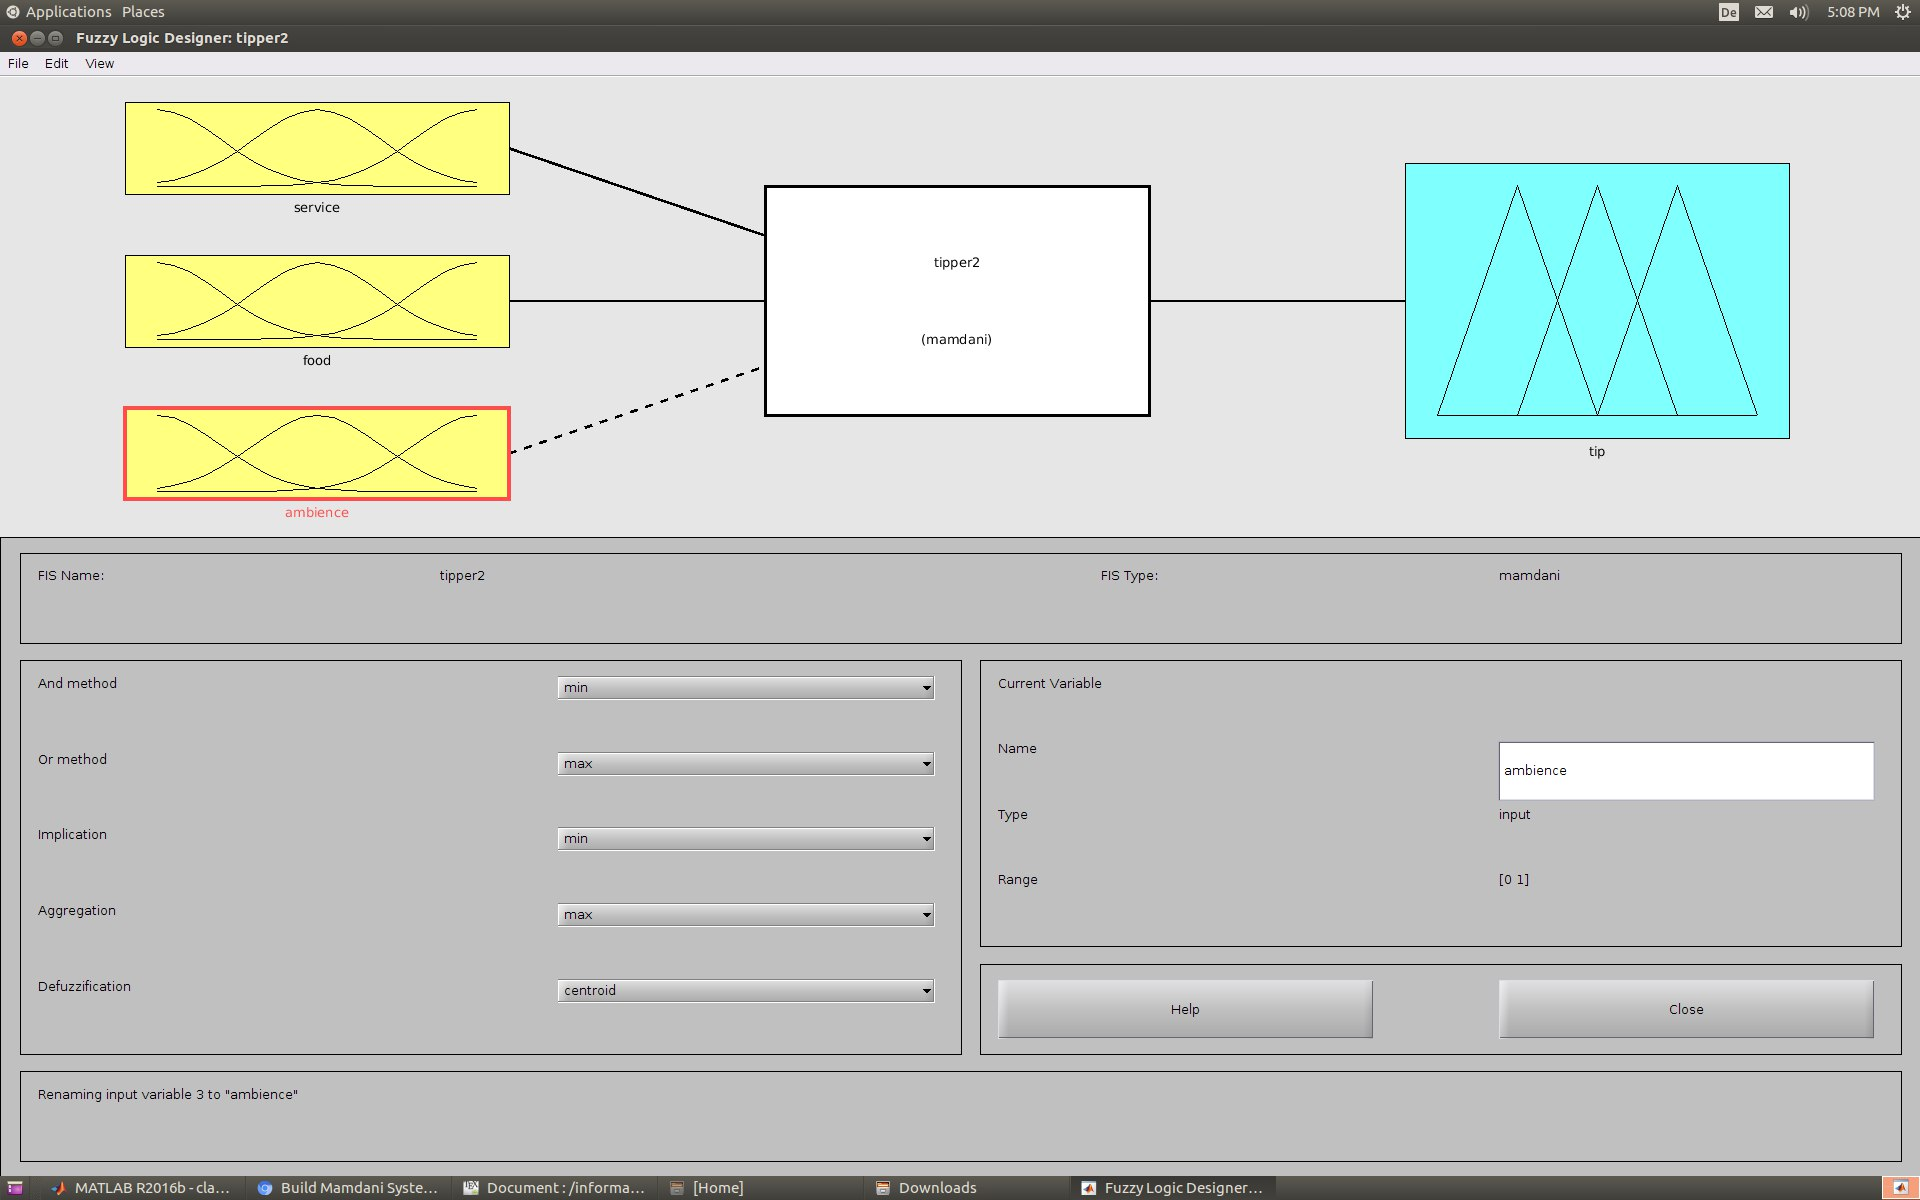
\includegraphics[scale=0.2]{ambience-added.jpg}
\end{figure}
Obviously, this new variable has no impact yet, since it has no membership functions and rules associated with it.

\newpage
\subsection{Selection of different membership functions}
Membership functions by input variable:\\
\textit{Service} has three membership functions; \textit{poor}, \textit{good} and \textit{excellent} which are centered around 0, 5 and 10 respectively. Each of these are gaussian functions which makes sense for such a diverse variable.\\
\textit{Food} has two membership functions; \textit{rancid} and \textit{delicious} which hold a plateau from 0 to 1 and from 9 to 10 respectively instead of centering around a maximum value like \textit{service}. This results in two radical sides with a big whole in the middle which represents a mediocre taste. This can make sense for food, because lots of people will usually gravitate towards extremes when it comes to the taste of their food.\\
A sensible way of including membership functions for our new variable \textit{ambience} could be this:

\begin{figure}[ht]
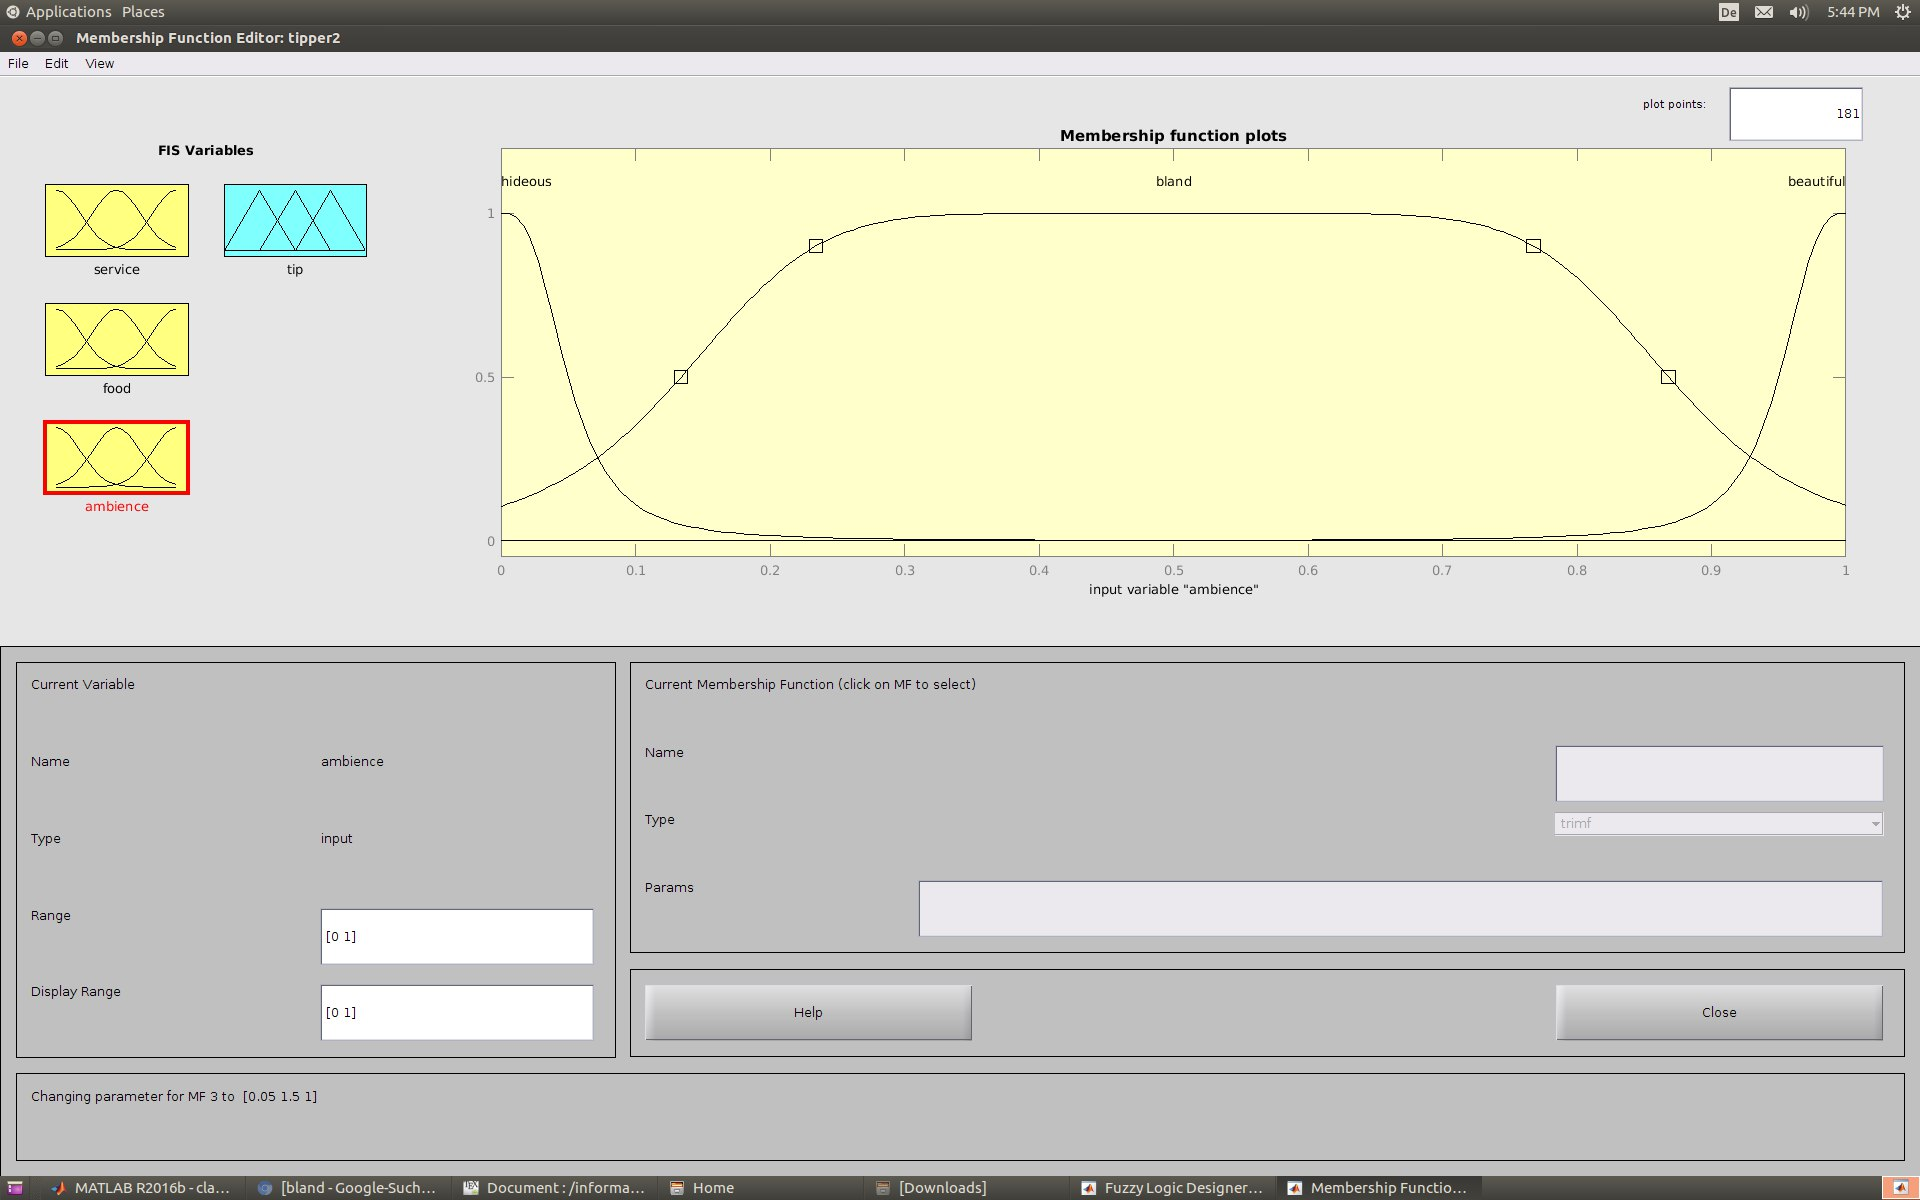
\includegraphics[scale=0.2]{ambience-mf.jpg}
\end{figure}

More picky for beautiful then for hideous, quite some overlap of bland with both ends, since bland can be hideous or beautiful sometimes, but REALLY bad and REALLY good usually means not really bland. bell for some reason.

\newpage
\subsection{Creation of rules}
Here is how rules were before:\\
Here is the changed look:

\begin{figure}[ht]
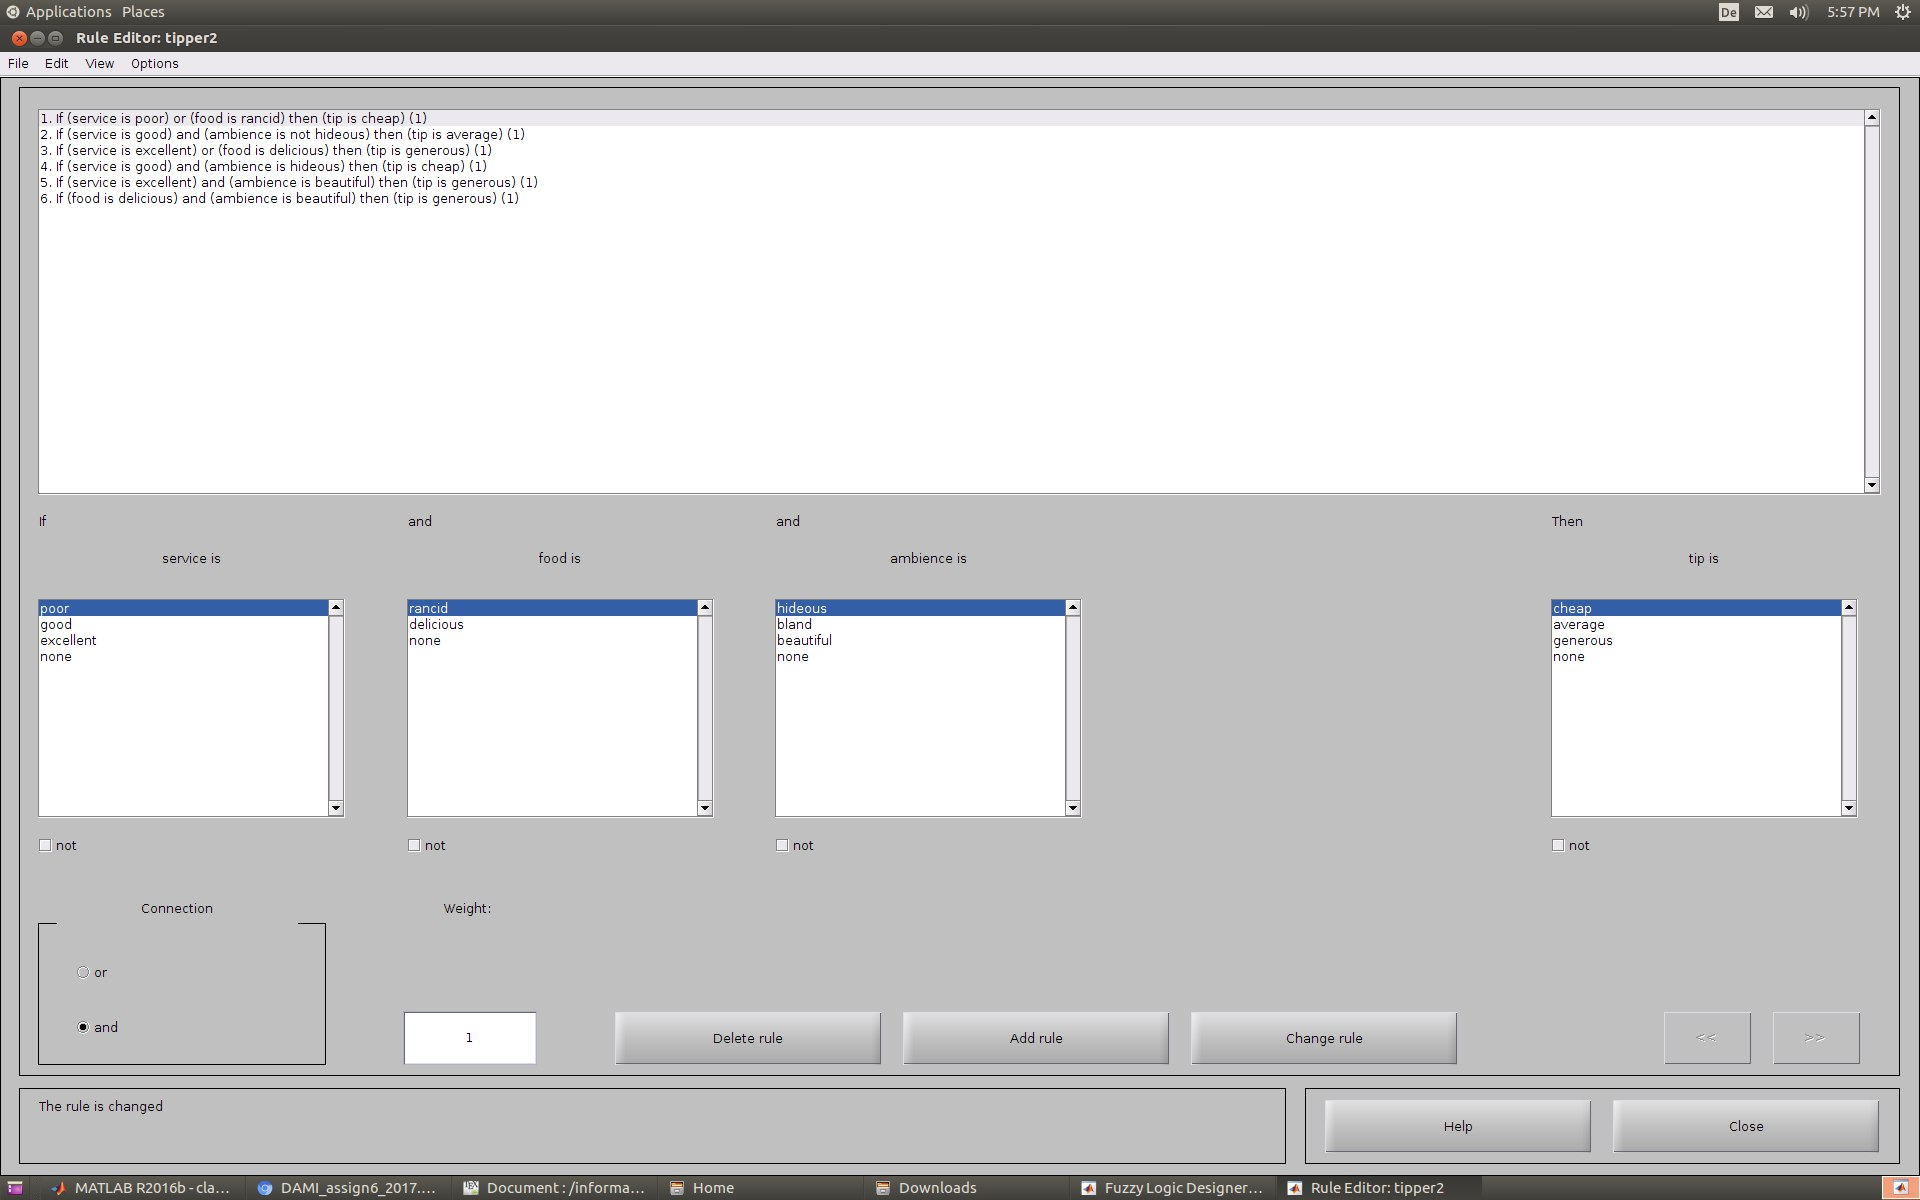
\includegraphics[scale=0.2]{ambience-rules.jpg}
\end{figure}

Here is my explaination:

\newpage
\subsection{Visualization}
Observation:\\
Change for pic (only pic of ambience to food and ambience to service since food to service is explained above):

\begin{figure}[ht]
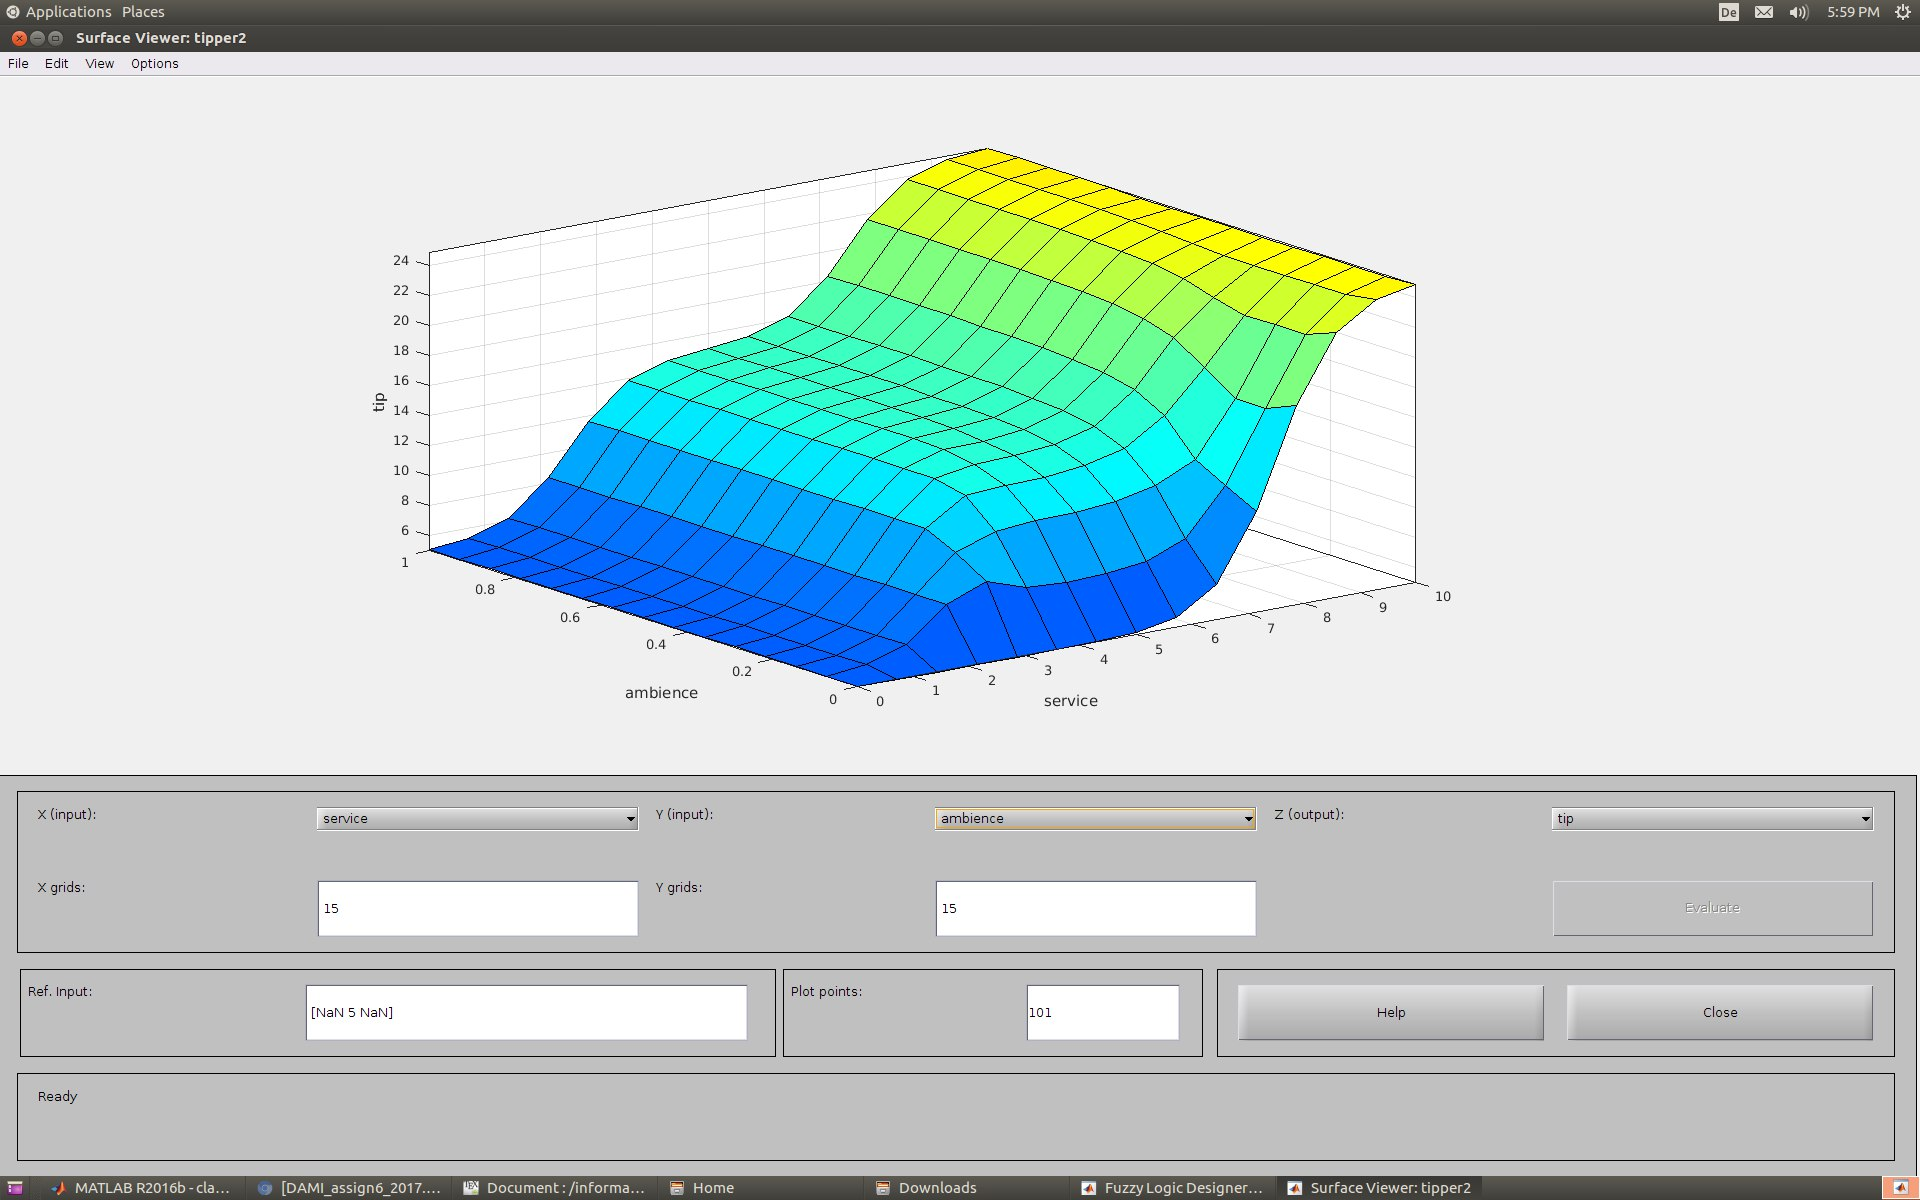
\includegraphics[scale=0.15]{ambience-surface-s.jpg}
\end{figure}

\begin{figure}[ht]
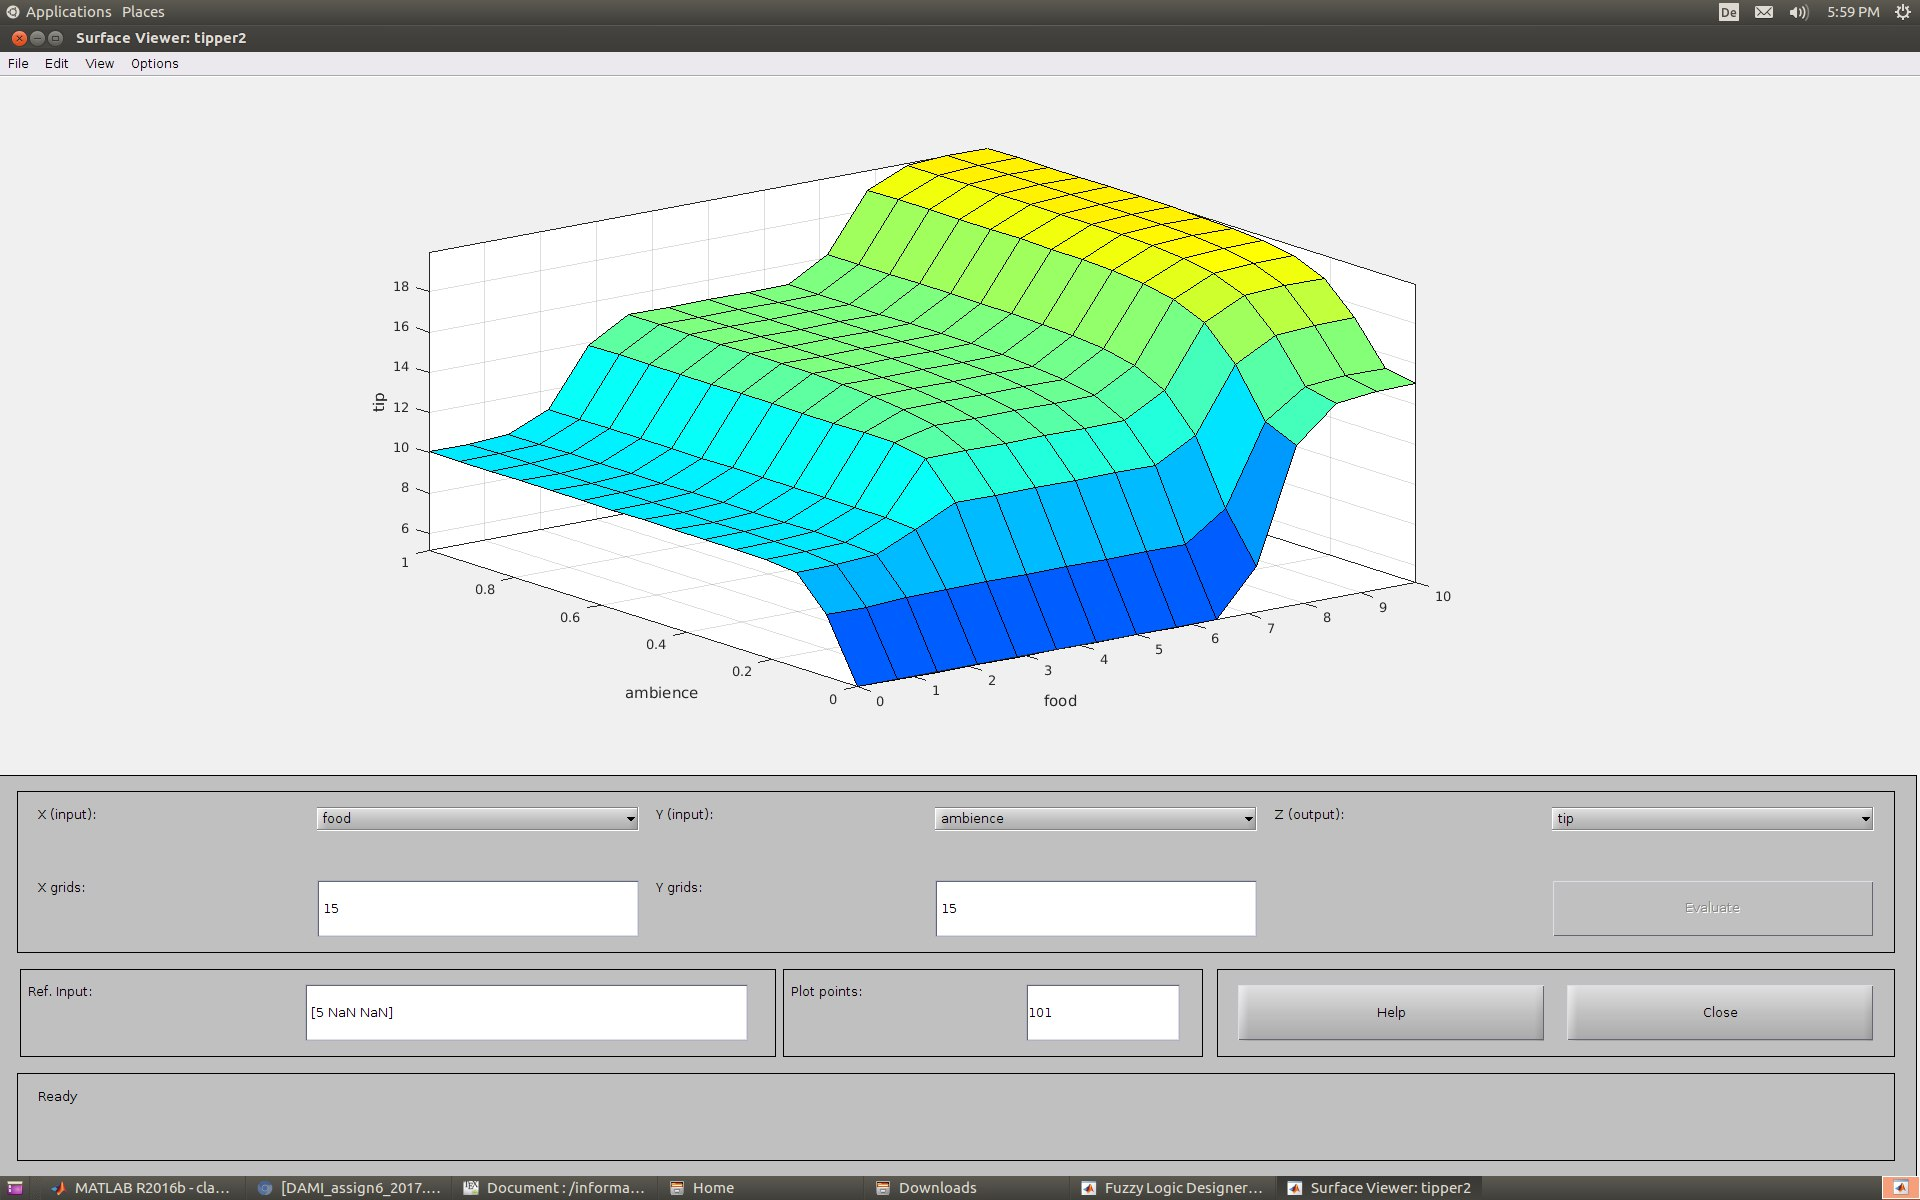
\includegraphics[scale=0.15]{ambience-surface-f.jpg}
\end{figure}

Change explain: some stuff

\newpage

\section{•}
Setup: we got a videogame reviewer. he judges based on these criteria: gameplay, story and originality. here are pics of all the graphs:
He rates gameplay above all else. As long as the game feels good to play, he will have fun with it and probably recommend the game to everybody.
Since he puts so much focus on gameplay, he has a lot of membership functions in the gameplay area, since he can judge poor from average from good from great etc
the other 2 factors, story and originality, he doesnt care too much for. for him, a good game doesnt have to excel in these areas. a game that is particularly bad
in one of those areas can also be elevated by having great gameplay. but even though he doesn't much care for these 2 areas, he isnt completely oblivious and a game
that is absolutely garbage in both of these areas will have a hard time being recommended even if the gameplay is pretty good
since he doesnt care that much about story and originality, he only judges them in extremes. as long as these areas arent completely garbage or absolutely amazing,
he mostly disregards them as "average".



\end{document}
